\section{Motivation}

\begin{frame}
  \frametitle{How slow is the vanilla program}
  \begin{block}{Setup}
    \begin{itemize}
    \item<+-> solar4k image
    \item<+-> encode 5 frames
    \end{itemize}
  \end{block}
  \onslide<+->
  \begin{exampleblock}{Hardware}
    \begin{itemize}
    \item Intel(R) Core(TM) i7-8750H CPU @ 2.20GHz
    \item NVIDIA GeForce GTX 1060 Mobile
    \end{itemize}
  \end{exampleblock}
  \onslide<+->
  \begin{alertblock}{Performance}
    \begin{itemize}
    \item The entire program: 808 s
    \end{itemize}
  \end{alertblock}
\end{frame}

\begin{frame}
  \frametitle{Callgraph of the vanilla program}
  \begin{figure}[h]
    \centering 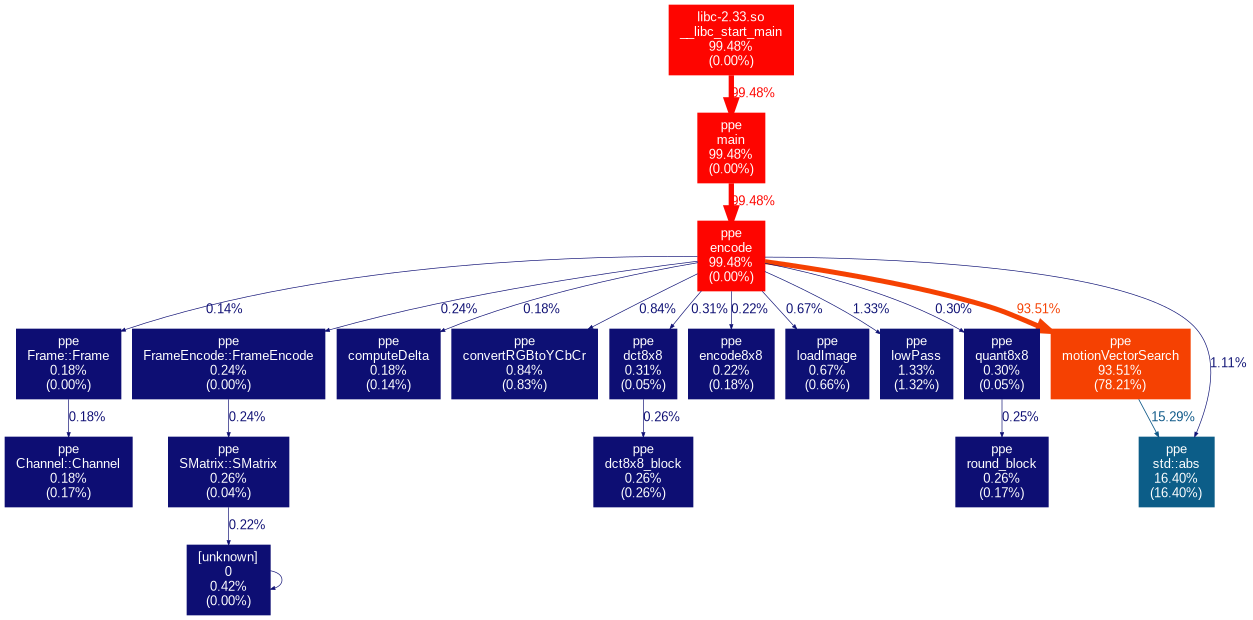
\includegraphics[height=6cm]{src/ppe-callgraph.png}
  \end{figure}
\end{frame}

\begin{frame}[fragile]
  \frametitle{Breakdown of the vanilla program}
  \begin{table}[h]
    \centering
    \begin{tabular}{ll}
      \toprule
      function & time (ms) \\
      \midrule
      \alert<4->{Convert to YCbCr} & \alert<4->{7000} \\
      \alert<3->{Low pass filter} & \alert<3->{10000} \\
      \alert<2->{Motion Vector Search} & \alert<2->{800000} \\
      Compute Delta &                1000 \\
      Downsample &                   1000 \\
      Convert to frequency domain &  3000 \\
      Quantize &                     2000 \\
      Compute DC differences &       50 \\
      Zig-zag order &                900 \\
      Encode coefficients &          3000 \\
      \midrule
      Total & 80000 \\
      \bottomrule
    \end{tabular}
  \end{table}
\end{frame}

%%% Local Variables:
%%% mode: latex
%%% TeX-master: "presentation"
%%% End:
